\documentclass[../main.tex]{subfiles}
\graphicspath{{\subfix{../figures/}}}
%
\begin{document}
\section{抽象工厂模式}
Abstract Factory

抽象工厂模式是所有形态的工厂模式中最为抽象和最具一般性的一种形态。抽象工厂模式的简略类图如下所示。
\begin{figure}[H]
  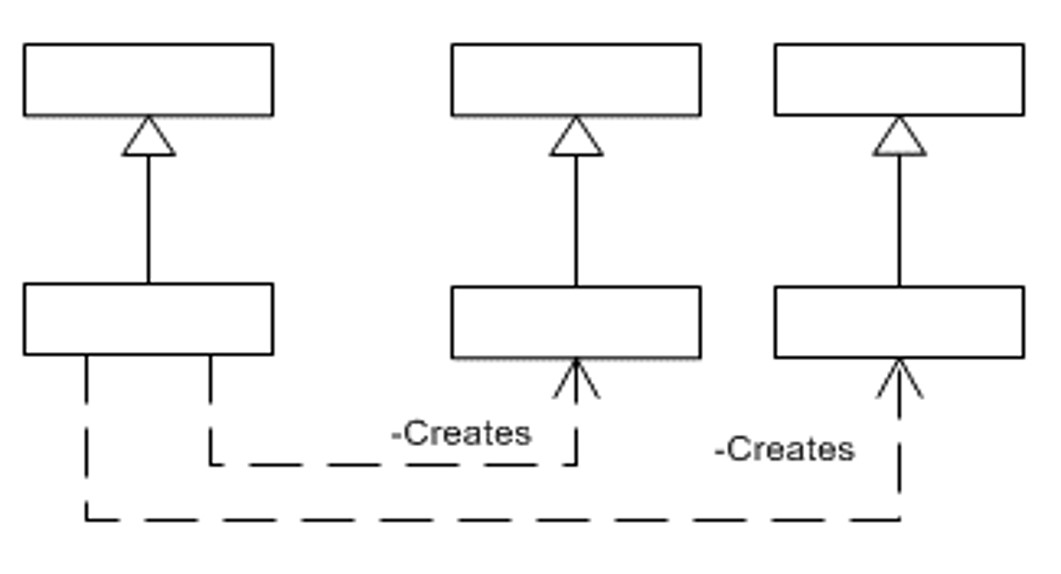
\includegraphics[width=0.55\textwidth]{17_1.jpg}
\end{figure}
%
抽象工厂模式面对的问题是多个产品继承结构的系统设计。
抽象工厂模式与工厂方法模式的最大区别就在于,工厂方法模式针对的是一个产品继承结构;而抽象工厂模式则需要面对多个产品继承结构。下图给出了一个产品继承结构。
\begin{figure}[H]
  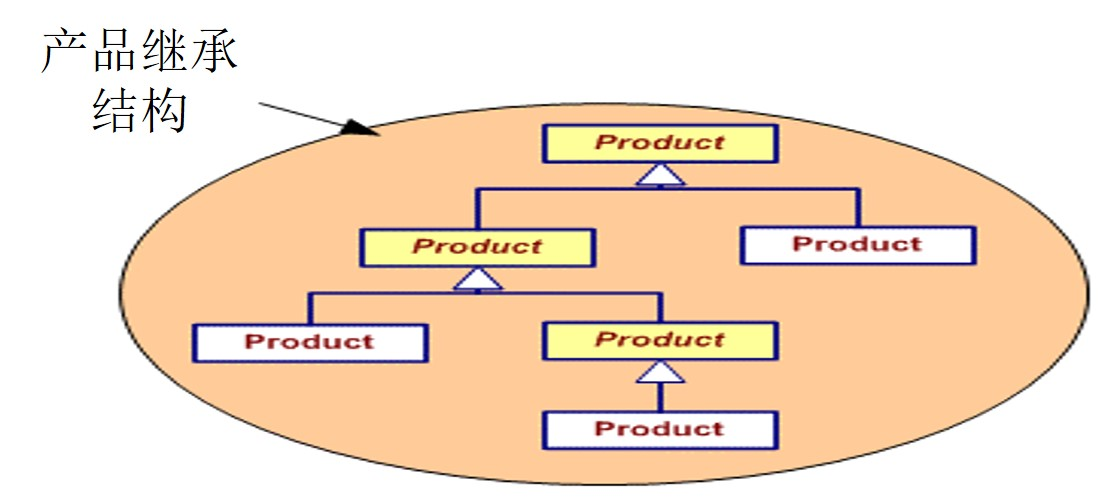
\includegraphics[width=0.55\textwidth]{17_2.jpg}
\end{figure}
%
下图则给出了多个相平行的产品继承结构的例子。
\begin{figure}[H]
  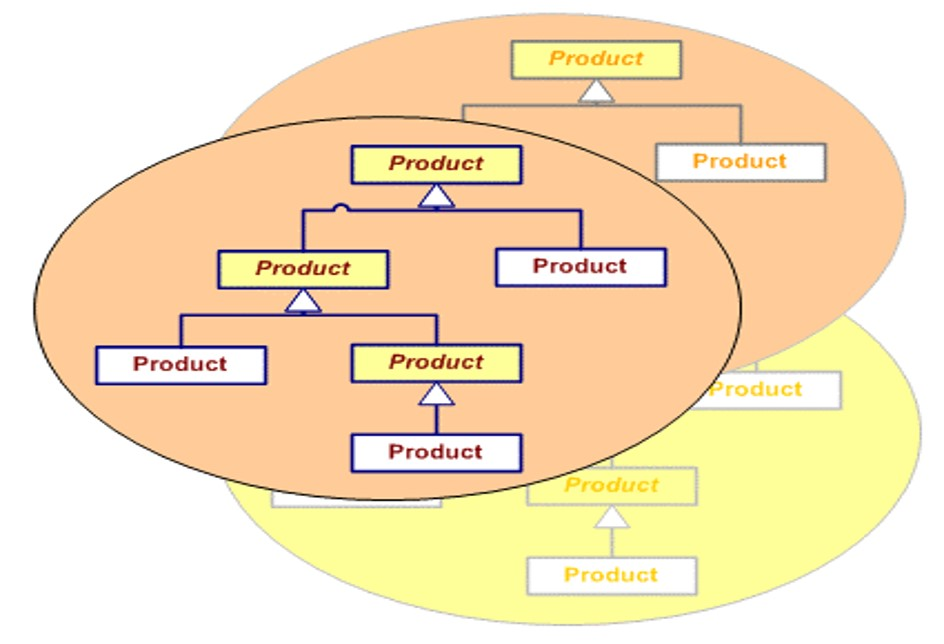
\includegraphics[width=0.55\textwidth]{17_3.jpg}
\end{figure}
%
为了方便引进抽象工厂模式,特地引进一个新的概念:\textbf{产品族}(Product Family)。所谓产品族,是指位于不同产品继承结构中,功能相关联的产品组成的家族。比如在下图中,箭头所指就是三个功能相关联的产品,它们位于三个不同的继承结构中的相同位置上,组成一个产品族。
\begin{figure}[H]
  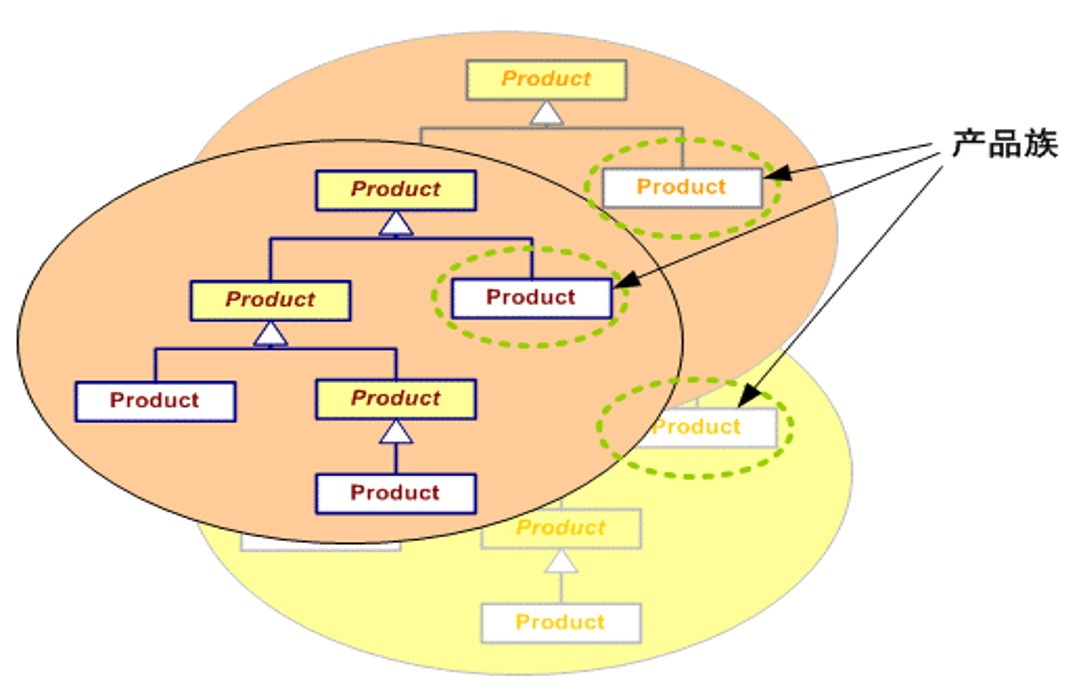
\includegraphics[width=0.55\textwidth]{17_4.jpg}
\end{figure}
显然,每一个产品族中含有产品的数目,与产品继承结构的数目是相等的。产品的继承结构和产品族将产品按照不同方向划分,形成一个二维的坐标系,如下图所示。
\begin{figure}[H]
  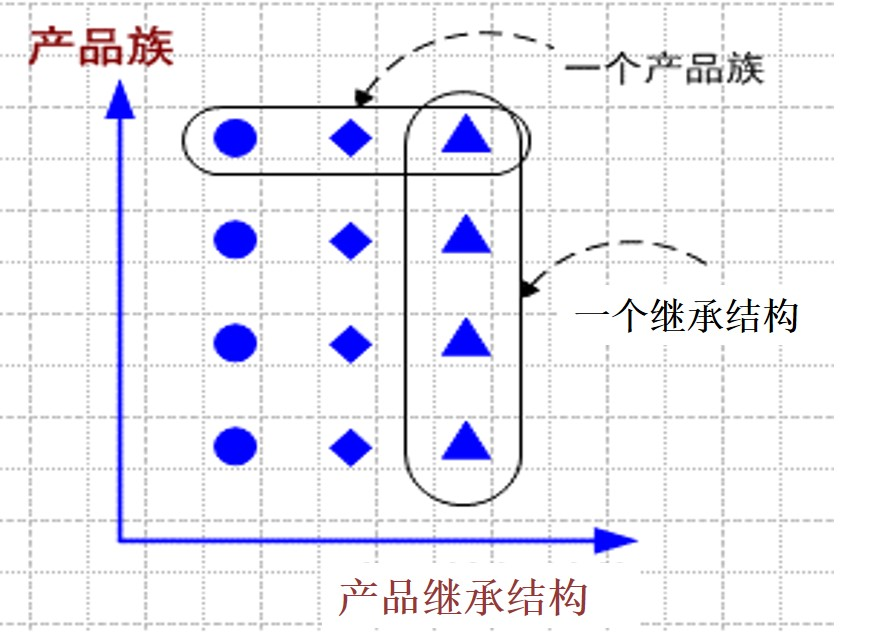
\includegraphics[width=0.55\textwidth]{17_5.jpg}
\end{figure}
%
在坐标图中有四个产品族,分布于三个产品继承结构中。
在上面的坐标图中,横轴表示产品继承结构,纵轴表示产品族。可以看出,图中一共有四个产品族,分布于三个不同的产品继承结构中。只要指明一个产品所处的产品族以及它所属的继承结构,就可以惟一地确定这个产品。

上面所给出的三个不同的继承结构具有平行的结构。因此,如果采用工厂方法模式,就势必要使用三个独立的工厂继承结构来对付这三个产品继承结构。由于这三个产品继承结构的相似性,会导致三个平行的工厂继承结构。随着产品继承结构的数目增加,工厂方法模式所给出的工厂继承结构的数目也会随之增加。
%
\begin{figure}[H]
  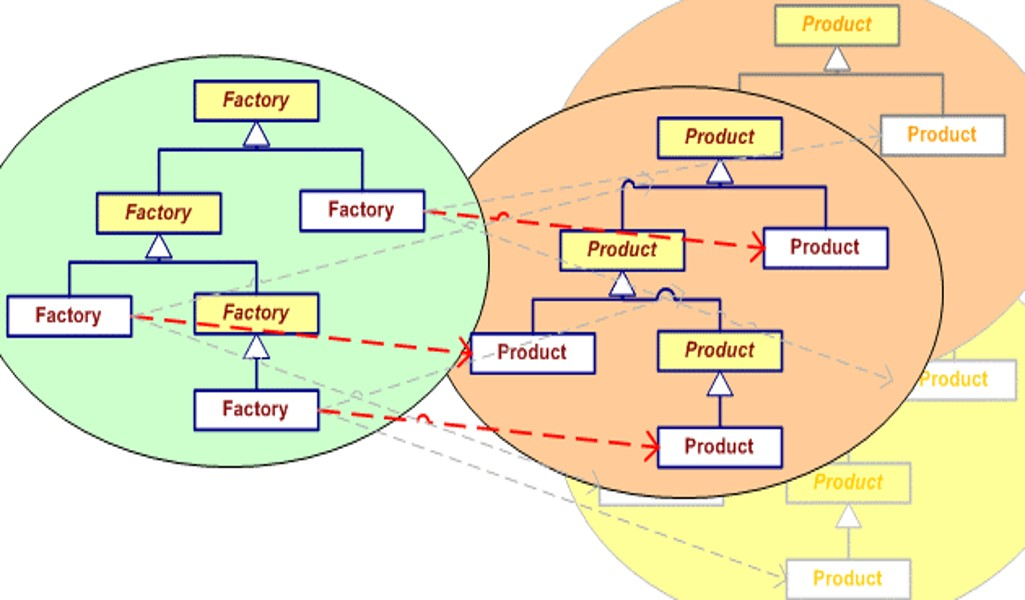
\includegraphics[width=0.55\textwidth]{17_6.jpg}
\end{figure}
%
可以看出,一个工厂继承结构可以创建出分属于不同产品继承结构的一个产品族中的所有对象;显然,这时候抽象工厂模式比工厂方法模式更有效率。
可以看出,对应于每一个产品族都有一个具体工厂。而每一个具体工厂负责创建属于同一个产品族、但是分属于不同继承结构的产品。
%
\begin{figure}[H]
  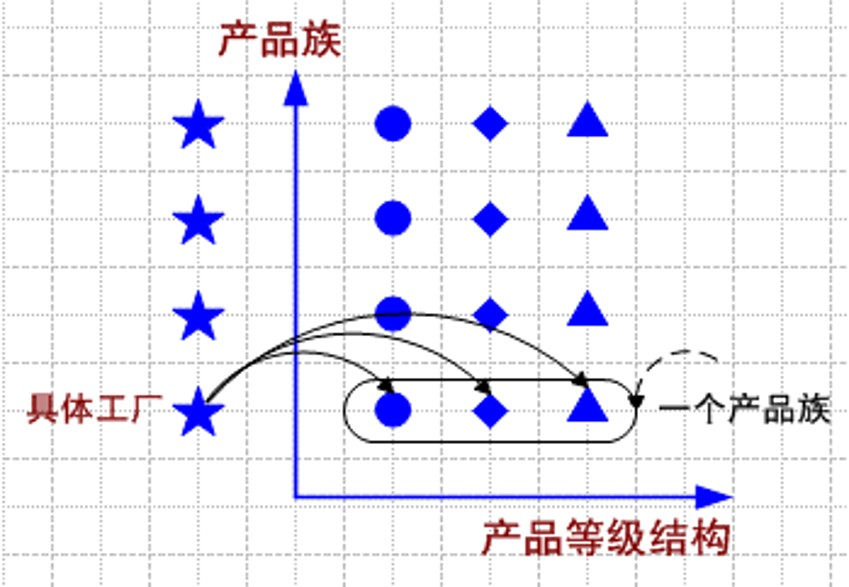
\includegraphics[width=0.55\textwidth]{17_7.jpg}
\end{figure}
%
\subsection{抽象工厂模式的结构}
通过使用抽象工厂模式,可以处理具有相同(或者相似)继承结构的多个产品族中的产品对象创建问题。比如下面就是两个具有相同继承结构的产品继承结构A 和产品继承结构B 的结构图。
\begin{figure}[H]
  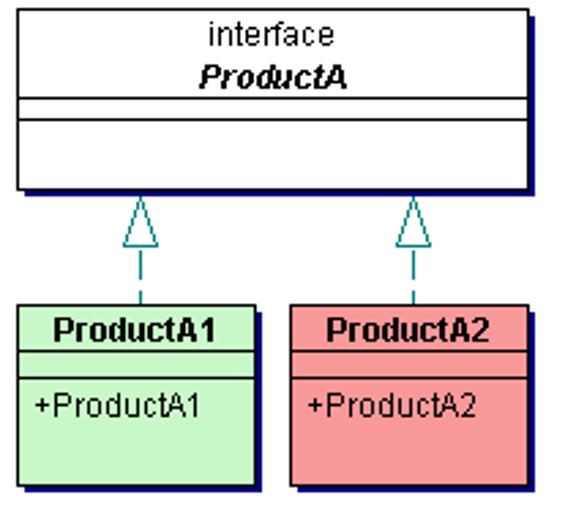
\includegraphics[width=0.40\textwidth]{17_8.jpg}
  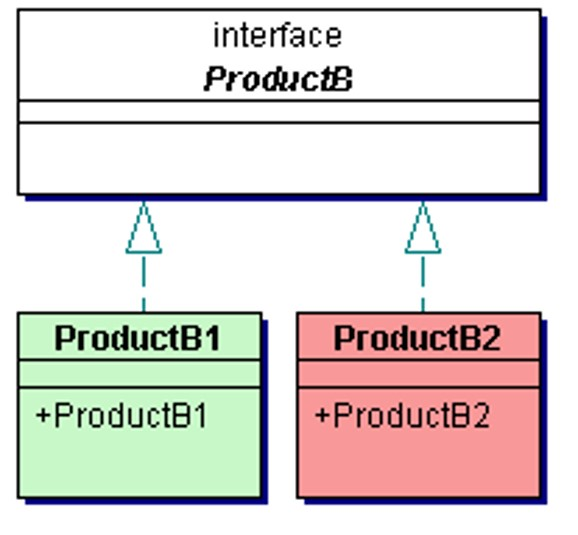
\includegraphics[width=0.40\textwidth]{17_9.jpg}
\end{figure}
%
如果使用坐标图描述的话,会看到在图上出现两个继承结构A 和B,以及两个产品族1 和2。如下图所示。
在下面的图中,每一个坐标点都代表一个具体产品角色。
\begin{figure}[H]
  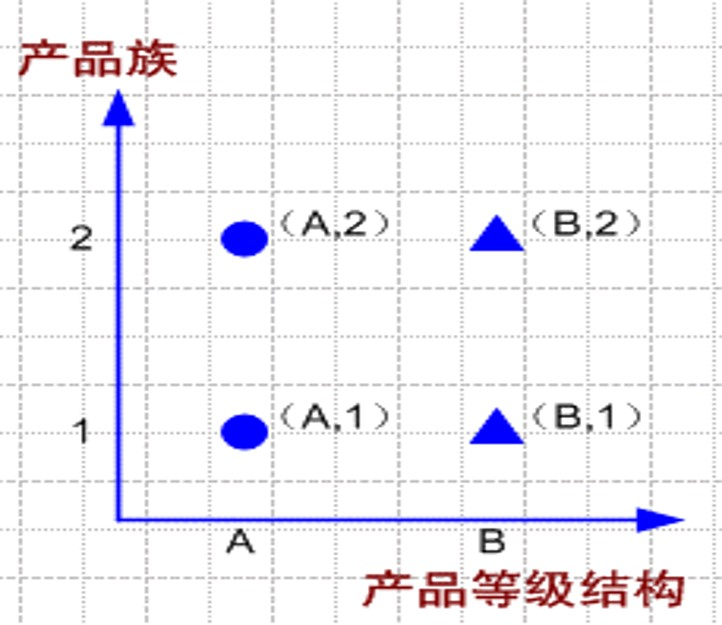
\includegraphics[width=0.50\textwidth]{17_10.jpg}
\end{figure}
%
如果使用工厂方法模式处理的话,就必须要有两个独立的工厂族。由于这两个产品族的继承结构相同,因此,使用同一个工厂族也可以处理这两个产品族的创建问题。后者就是抽象工厂模式,这样根据产品角色的结构图,就不难给出工厂角色的结构设计图,如下图所示。
\begin{figure}[H]
  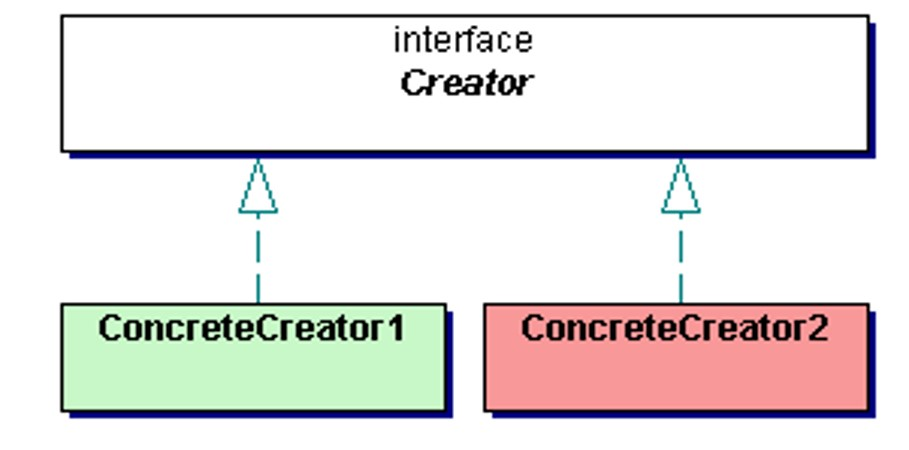
\includegraphics[width=0.50\textwidth]{17_11.jpg}
\end{figure}
%
由于每个具体工厂角色都需要负责两个不同继承结构的产品对象的创建,因此每个工厂角色都需要提供两个工厂方法,分别用于创建两个继承结构的产品。既然每个具体工厂角色都需要实现这两个工厂方法,所以这种情况就具有一般性,不妨抽象出来,移动到抽象工厂角色Creator 中加以声明。产品继承结构A 和产品继承结构B 的结构图如下所示。
可以看出,每一个工厂角色都有两个工厂方法,分别负责创建分属不同产品继承结构的产品对象。
\begin{figure}[H]
  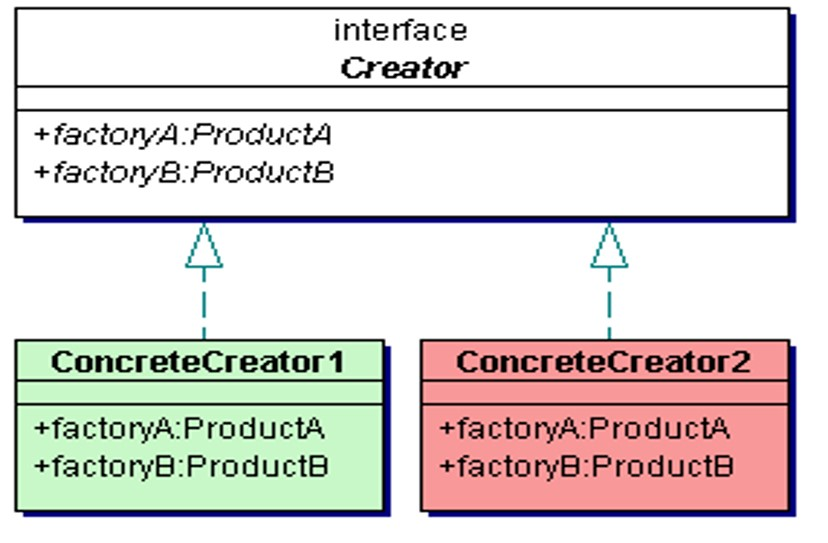
\includegraphics[width=0.50\textwidth]{17_12.jpg}
\end{figure}
%
采用抽象工厂模式设计出的系统类图如下所示。
\begin{figure}[H]
  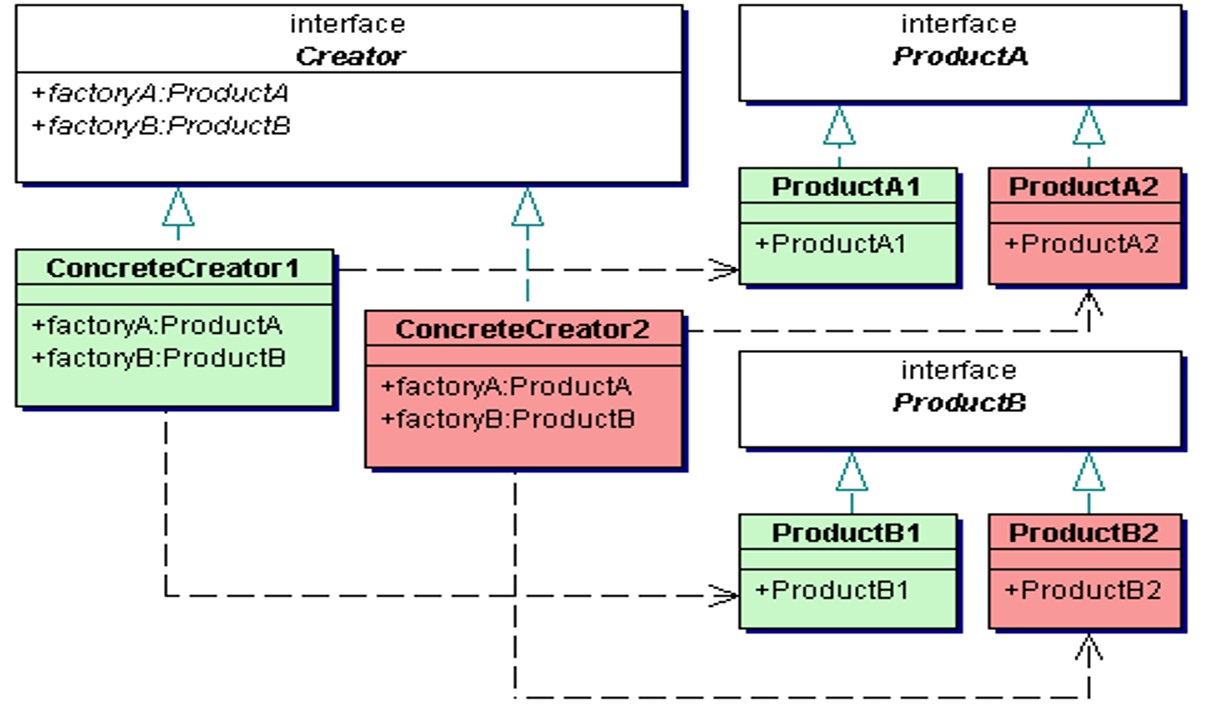
\includegraphics[width=0.65\textwidth]{17_13.jpg}
\end{figure}
%
从上图可以看出,抽象工厂模式涉及到以下的角色。
\begin{itemize}
  \item 抽象工厂(Abstract Factory)角色:担任这个角色的是抽象工厂模式的核心,它是与应用系统的业务逻辑无关的。通常使用Java 接口或者抽象Java 类实现,而所有的具体工厂类必须实现这个Java 接口或继承这个抽象Java 类。
  \item 具体工厂类(Concrete Factory)角色:这个角色直接在客户端的调用下创建产品的实例。这个角色含有选择合适的产品对象的逻辑,而这个逻辑是与应用系统的业务逻辑紧密相关的。通常使用具体Java 类实现这个角色。
  \item 抽象产品(Abstract Product)角色:担任这个角色的类是抽象工厂模式所创建的对象的父类,或它们共同拥有的接口。通常使用Java 接口或者抽象Java 类实现这一角色。
  \item 具体产品(Concrete Product)角色:抽象工厂模式所创建的任何产品对象都是某一个具体产品类的实例。这是客户端最终需要的东西,其内部一定实现了应用系统的业务逻辑。通常使用具体Java 类实现这个角色。
\end{itemize}
%
首先给出工厂角色的源代码,可以看出,抽象工厂角色规定出两个工厂方法,分别提供两个不同继承结构的产品对象。
\begin{lstlisting}[language=java]
public interface Creator {
  // 产品继承结构A 的工厂方法
  public ProductA factoryA();
  // 产品继承结构B 的工厂方法
  public ProductB factoryB();
}
\end{lstlisting}
%
\noindent 下面给出具体工厂角色ConcreteCreator1 的源代码。这个具体工厂类实现了抽象工厂角色所要求的两个工厂方法,分别提供两个产品继承结构中的某一个产品对象。
%
\begin{lstlisting}[language=java]
public class ConcreteCreator1 implements Creator {
  // 产品继承结构 A 的工厂方法
  public ProductA factoryA() { return new ProductA1(); }
  // 产品继承结构 B 的工厂方法
  public ProductB factoryB() { return new ProductB1(); }
}
\end{lstlisting}
%
一般而言,有多少个产品继承结构,在工厂角色中就有对应个数的个工厂方法。每一个产品继承结构中有多少具体产品,就有多少个产品族,也就会在工厂继承结构中发现多少个具体工厂。

下面给出具体工厂角色ConcreteCreator2 的源代码。这个具体工厂类实现了抽象工厂角色所要求的两个工厂方法,分别提供两个产品继承结构中的另一个产品对象。
\begin{lstlisting}[language=java]
public class ConcreteCreator2 implements Creator {
  // 产品继承结构A 的工厂方法
  public ProductA factoryA() { return new ProductA2(); }
  // 产品继承结构B 的工厂方法*/
  public ProductB factoryB() { return new ProductB2(); }
}

public interface ProductA {  }
public class ProductA1 implements ProductA {  }
public class ProductA2 implements ProductA {  }

public interface ProductB {  }
public class ProductB1 implements ProductB {  }
public class ProductB2 implements ProductB {  }
\end{lstlisting}
%
\textbf{在以下情况下应当考虑使用抽象工厂模式}:
\begin{enumerate}
  \item 一个系统不应当依赖于产品类实例如何被创建、组合和表达的细节。这对于所有形态的工厂模式都是重要的;
  \item 这个系统的产品有多于一个的产品族,而系统只消费其中某一族的产品;
  \item 同属于同一个产品族的产品是在一起使用的,这一约束必须要在系统的设计中体现出来;
\end{enumerate}
%
\subsection{抽象工厂模式的应用}
\noindent 抽象工厂模式的起源或者说最早的应用,是用于创建分属于不同操作系统的视窗构件。比如,命令按键(Button)与文字框(Text)都是视窗构件,在UNIX 操作系统的视窗环境和Windows 操作系统的视窗环境中,这两个构件有不同的本地实现,它们的细节也有所不同。

\noindent 在每一个操作系统中,都有一个视窗构件组成的构件家族。在这里就是Button 和Text组成的产品族。而每一个视窗构件都构成自己的继承结构,由一个抽象角色给出抽象的功能描述,而由具体子类给出不同操作系统下的具体实现,如下图所示。
\begin{figure}[H]
  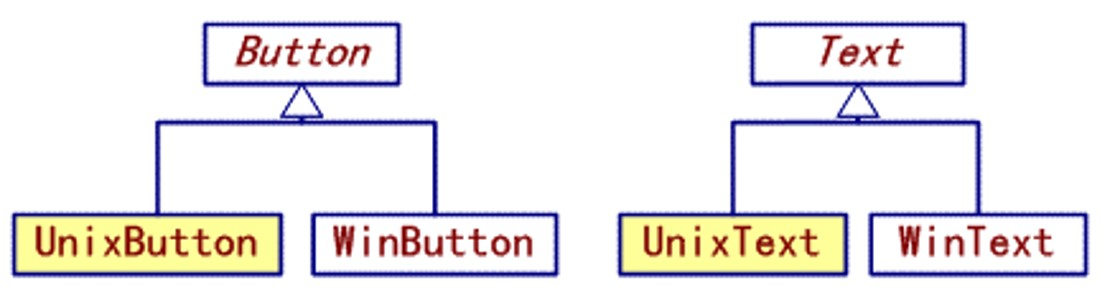
\includegraphics[width=0.50\textwidth]{17_14.jpg}
\end{figure}
%
可以发现在上面的产品类图中,有两个产品的继承结构,分别是Button 继承结构和Text继承结构。同时有两个产品族,也就是UNIX 产品族和Windows 产品族。UNIX 产品族由UnixButton 和UnixText 产品构成;而Windows 产品族由WinButton 和WinText 产品构成。
%
\begin{figure}[H]
  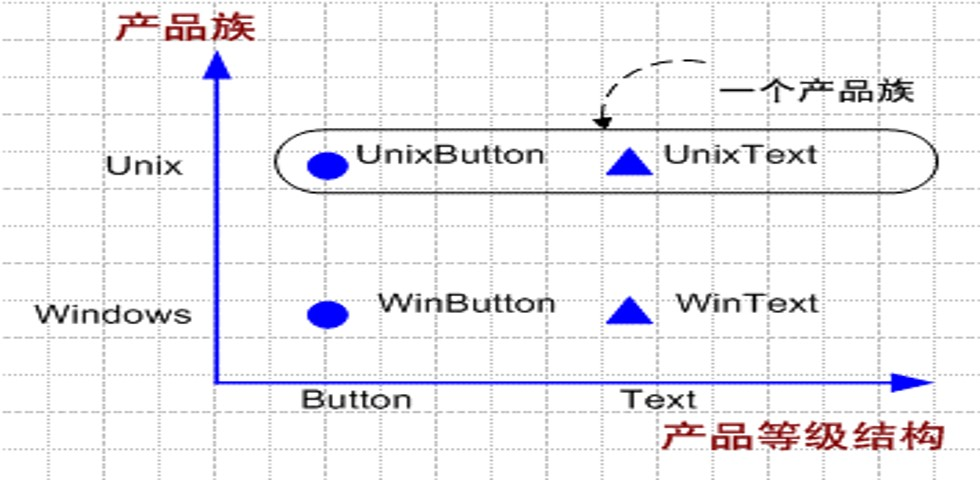
\includegraphics[width=0.50\textwidth]{17_15.jpg}
  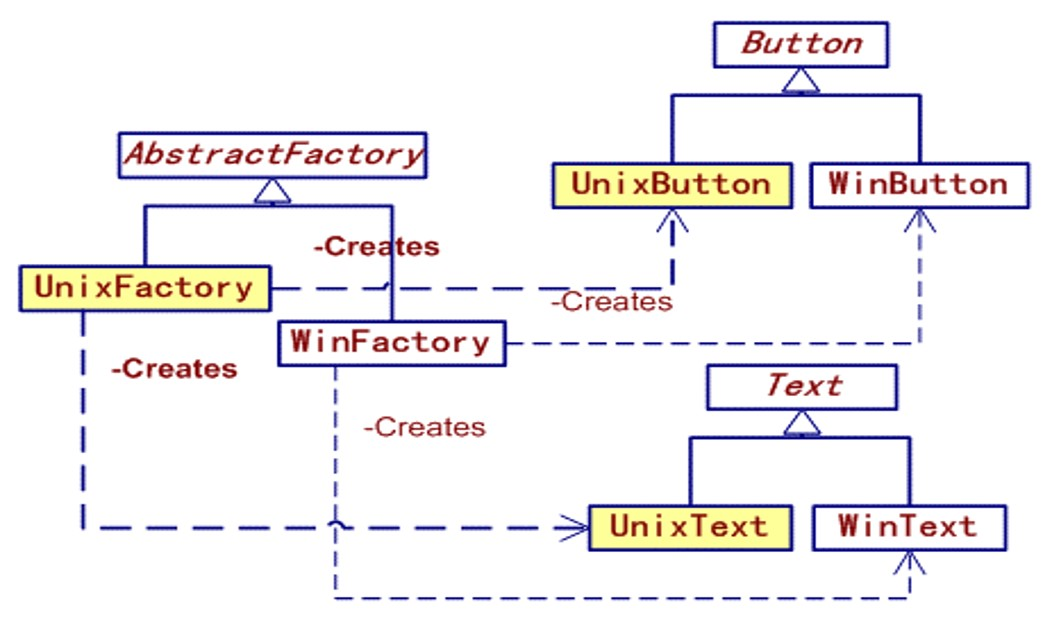
\includegraphics[width=0.50\textwidth]{17_16.jpg}
\end{figure}
%
系统对产品对象的创建需求由一个工厂的继承结构满足;其中有两个具体工厂角色,即UnixFactory 和WinFactory。其中UnixFactory 对象负责创建Unix 产品族中的产品,而WinFactory 对象负责创建Windows 产品族中的产品。这就是抽象工厂模式的应用,抽象工厂模式的解决方案如图所示。
%
\begin{lstlisting}[language=java]
abstract class Button {
  public abstract void paint();
}

class WinButton extends Button  {
  public void paint()    {
    System.out.println("I'm a WinButton");
  }
}

class OSXButton extends Button {
  public void paint() {
    System.out.println("I'm an OSXButton");
  }
}

abstract class GUIFactory {
  public static GUIFactory getFactory() {
    //从配置文件中读取操作系统类型
    int sys = readFromConfigFile("OS_TYPE");
    if (sys == 0) {
      return new WinFactory();
    } else {
      return new OSXFactory();
    }
  }
   public abstract Button createButton();
}

//生成Windows界面的工厂
class WinFactory extends GUIFactory {
  public Button createButton() { return new WinButton(); }
}

//生成OS X界面的工厂
class OSXFactory extends GUIFactory {
  public Button createButton() { return new OSXButton(); }
}

public class Application {
  public static void main(String[] args) {
    GUIFactory factory = GUIFactory.getFactory();
    Button button = factory.createButton();
    button.paint();
  }
}
\end{lstlisting}
%
\subsection{抽象工厂模式在农场系统中的实现}
农场公司再次面临新的大发展,一项重要的工作,就是引进塑料大棚技术,在大棚里种植热带(Tropical)和北方的水果和蔬菜。
因此,在这个系统里面,产品分成两个继承结构:水果(Fruit)和蔬菜(Veggie)。下面就是水果(Fruit)的类图。
\begin{figure}[H]
  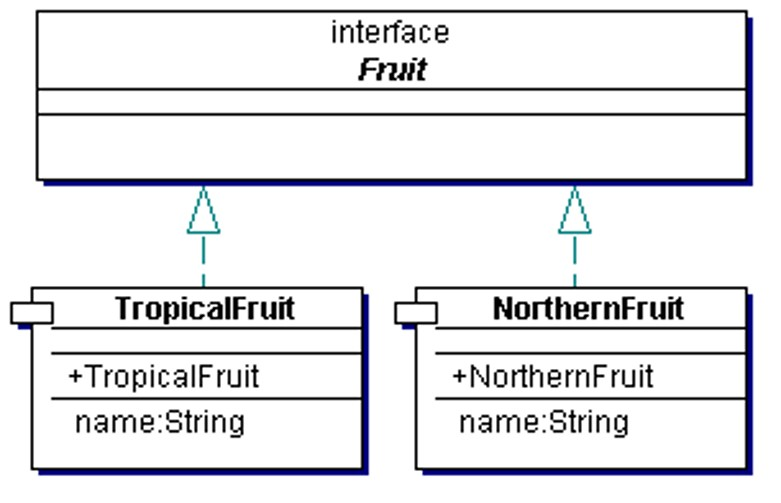
\includegraphics[width=0.50\textwidth]{17_17.jpg}
\end{figure}
%
下面则是蔬菜(Veggie)的类图。
\begin{figure}[H]
  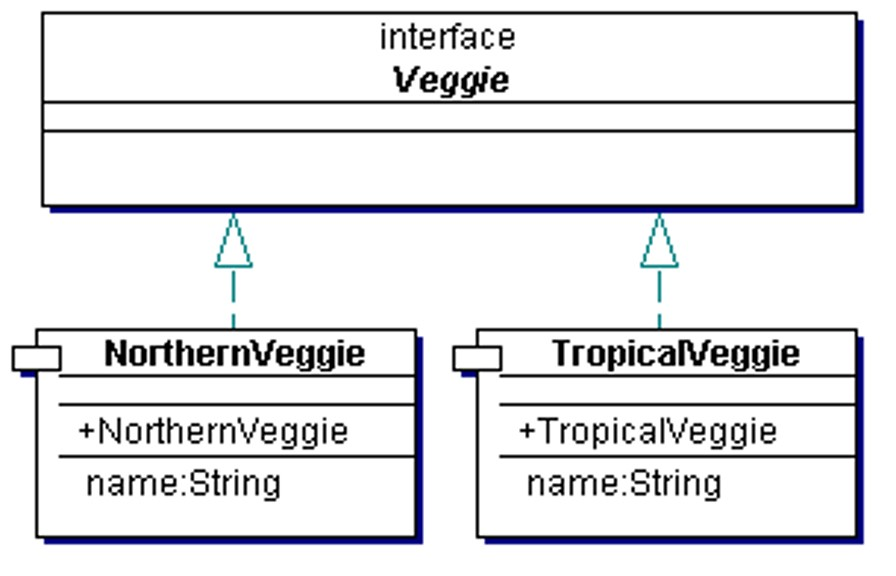
\includegraphics[width=0.50\textwidth]{17_18.jpg}
\end{figure}
%
下面是描述这个系统的产品角色的相图。
\begin{figure}[H]
  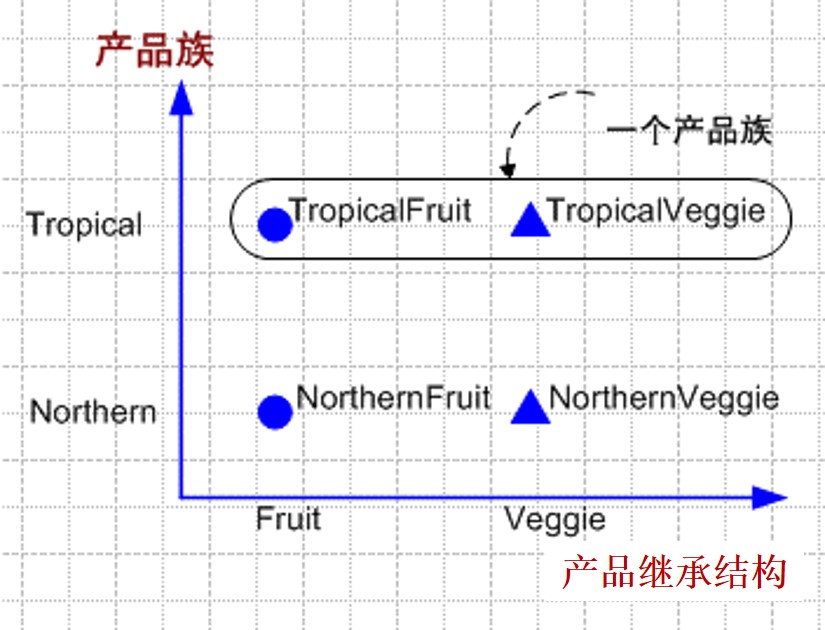
\includegraphics[width=0.50\textwidth]{17_19.jpg}
\end{figure}
%
可以看出,这个系统的产品可以分成两个继承结构:Fruit 和Veggie,以及两个产品族:Tropical 和Northern。坐标图上出现了四个坐标点,分别代表TropicalFruit(热带水果)、TropicalVeggie(热带蔬菜)、NorthernFruit(北方水果)以及NorthernVeggie(北方蔬菜)等四个产品。
显然可以使用一个工厂族来封装它们的创建过程。这个工厂族的继承结构应当与产品族的继承结构完全平行,园丁继承结构的类图如下图所示。
系统所需要的是产品的实例,而工厂则是对产品创建过程的封装。

\textbf{系统设计}:与抽象工厂模式的各个角色相对照,不难发现,所谓各个园丁其实就是各个工厂角色,而蔬菜和水果角色则是产品角色。将抽象工厂模式应用于农场系统中,系统的设计图如下所示。
\begin{figure}[H]
  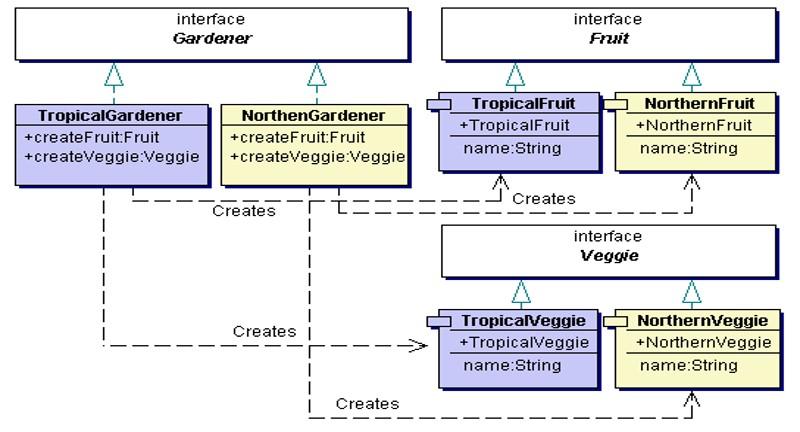
\includegraphics[width=0.70\textwidth]{17_20.jpg}
\end{figure}
%
种在田间的北方作物与种在大棚的热带作物都是系统的产品,它们分属于两个产品族。显然,北方作物是要种植在一起的,而大棚作物是要另外种植在一起的。这些分别体现在系统的设计上,就正好满足了使用抽象工厂模式的第三个条件。
\begin{lstlisting}[language=java]
// 抽象工厂类
public interface Gardener {
  public Fruit creatFruit();
  public Veggie createVeggie();
}

// 具体工厂类
public class NorthernGardener implements Gardener {
  // 水果的工厂方法
  public Fruit createFruit(String name) {
    return new NorthernFruit(name);
  }
  // 蔬菜的工厂方法
  public Veggie createVeggie(String name) {
    return new NorthernVeggie(name);
  }
}

// 具体工厂类
public class TropicalGardener implements Gardener {
  // 水果的工厂方法
  public Fruit createFruit(String name) {
    return new TropicalFruit(name);
  }
  // 蔬菜的工厂方法
  public Veggie createVeggie(String name) {
    return new TropicalVeggie(name);
  }
}

public interface Veggie {}

// 具体产品类
public class NorthernVeggie implements Veggie{
  private String name;
  public NorthernVeggie(String name) {  }
  public String getName() { return name; }
  public void setName(String name) { this.name = name; }
}

// 具体产品类
public class TropicalVeggie implements Veggie {
  private String name;
   public TropicalVeggie(String name) { this.name = name; }
   public String getName() { return name; }
   public void setName(String name) { this.name = name; }
}

public interface Fruit {  }

public class NorthernFruit implements Fruit {
  private String name;
  public NorthernFruit(String name) {  }
  public String getName() { return name; }
   public void setName(String name) { this.name = name; }
}

public class TropicalFruit implements Fruit {
  private String name;
  public TropicalFruit(String name) {  }
  public String getName() { return name; }
  public void setName(String name) { this.name = name; }
}
// 在使用时,客户端只需要创建具体工厂的实例,
// 然后调用工厂对象的工厂方法,就可以得到所需要的产品对象。
\end{lstlisting}
%
\subsection{开闭原则}
开闭原则要求一个软件系统可以在不修改原有代码的情况下,通过扩展达到增强其功能的目的。对于一个涉及到多个产品继承结构和多个产品族的系统,其功能的增强不外乎两个方面:
\begin{itemize}
  \item 增加新的产品族;
  \item 增加新的产品继承结构。
\end{itemize}
那么抽象工厂模式是怎样支持这两方面功能增强的呢?
\begin{itemize}
  \item 增加新的产品族:只需要向系统中加入新的具体工厂类就可以了,没有必要修改已有的工厂角色或者产品角色。因此,在系统中的产品族增加时,抽象工厂模式是支持开闭原则的。
  \item 增加新的产品继承结构:需要修改所有的工厂角色,给每一个工厂类都增加一个新的工厂方法,而这显然是违背开闭原则的。换言之,对于产品继承结构的增加,抽象工厂模式是不支持开闭原则的。
\end{itemize}
综合起来,抽象工厂模式以一种倾斜的方式支持增加新的产品,它为新产品族的增加提供方便,而不能为新的产品继承结构的增加提供这样的方便。
\end{document}
